\chapter*{Felhasználói dokumentáció}

\section*{Az alkalmazás futtatásához szükséges alapvető tudnivalók}

A futtatáshoz szükséges alapvető rendszerkövelmények:
\begin{itemize}
\item OS: Windows 7 SP1+
\item Videókártya: DX9 (shader model 3.0) vagy DX11 feature level 9.3 +
\item CPU: SSE2 utasításkészlet  támogatás.
\end{itemize}

\noindent A program futtatásához nincs szükség telepítésre, csak a futtatható állományra és egyéb függőségekre, amik mellékelve vannak.
\newline
\newline Szükséges állományok:
\begin{cpp}
Szakdolgozat.exe Assembly-CSharp.dll Mono.Security.dll mscorlib.dll
System.Core.dll System.dll UnityEngine.dll UnityEngine.Networking.dll
UnityEngine.PlaymodeTestsRunner.dll UnityEngine.UI.dll
UnityEngine.dll.mdb mono.dll MonoPosixHelper.dll settings.map
DefaultWsdlHelpGenerator.aspx machine.config Compat.browser
web.config config.xml browscap.ini  unity\_builtin\_extra app.info 
globalgamemanagers unity\_default\_resources
globalgamemanagers.assets level0 sharedassets0.assets
\end{cpp}

\section*{Használat}
A programot a \texttt{Szakdolgozat.exe} futtatható állomány megnyitásával indíthatjuk el, ami után a \ref{fig:UnityStartUp}. ábrán látható ablak fogad minket.

\begin{figure}[h!]
\centering
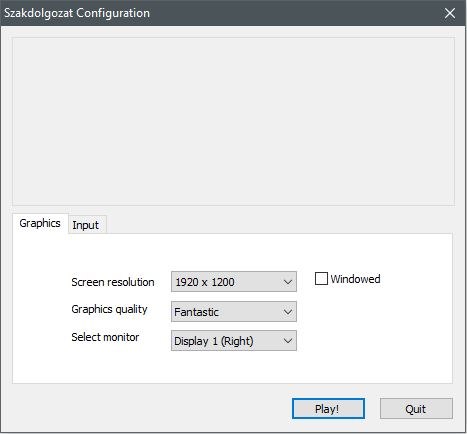
\includegraphics[scale=0.5]{kepek/UnityStartUp.jpg}
\caption{A program grafikai beállítási lehetőségei}
\label{fig:UnityStartUp}
\end{figure}

Itt van lehetőségünk a különböző grafikai beállításokat módosítani. Beállíthatjuk a kívánt felbontást, hogy teljes képernyős módban fusson az alkalmazás vagy ne. A grafikai beállítás leginkább a fényekre és az árnyékokra van hatással. Maximális beállítások mellett valósidejű árnyékokat generál az alkalmazás, viszont minimális beállítások mellett kikapcsolja az árnyékokat. Ezért nagyobb méretű térképek generálásakor vagy gyengébb specifikációjú rendszerek esetén érdemes az alacsonyabb grafikai beállításokat választani.

A \ref{fig:UserGuide1}. ábrán látható a generálás előtti felhasználói felület, a \ref{fig:UserGuide2}. ábrán pedig a generálás utáni állapot. Ahogy az ábrákon látható nem minden beállítási lehetőség módosítható a generálás után, csak a hőmérsékletet lehet befolyásolni utólag. A térkép generálásához 10 különböző beállítási lehetőség tartozik.

\begin{figure}[h!]
\centering
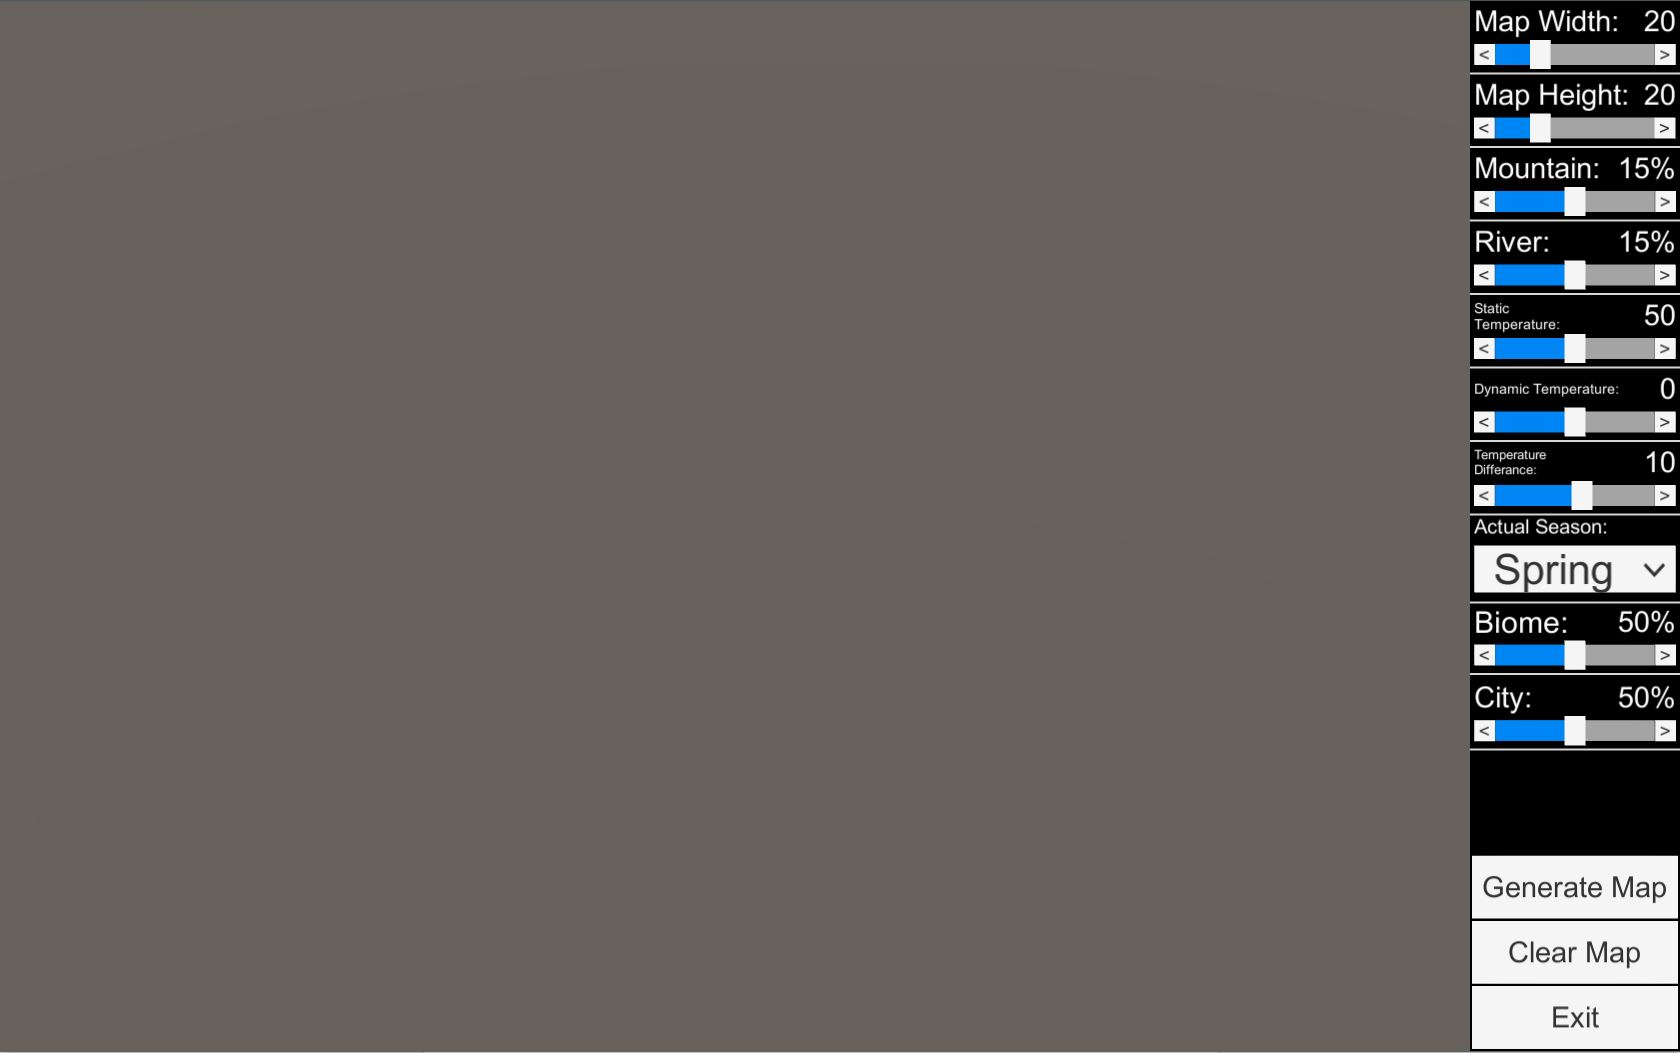
\includegraphics[scale=0.215]{kepek/UserGuide1.jpg}
\caption{A program grafikai beállítási lehetőségei}
\label{fig:UserGuide1}
\end{figure}

\begin{figure}[h!]
\centering
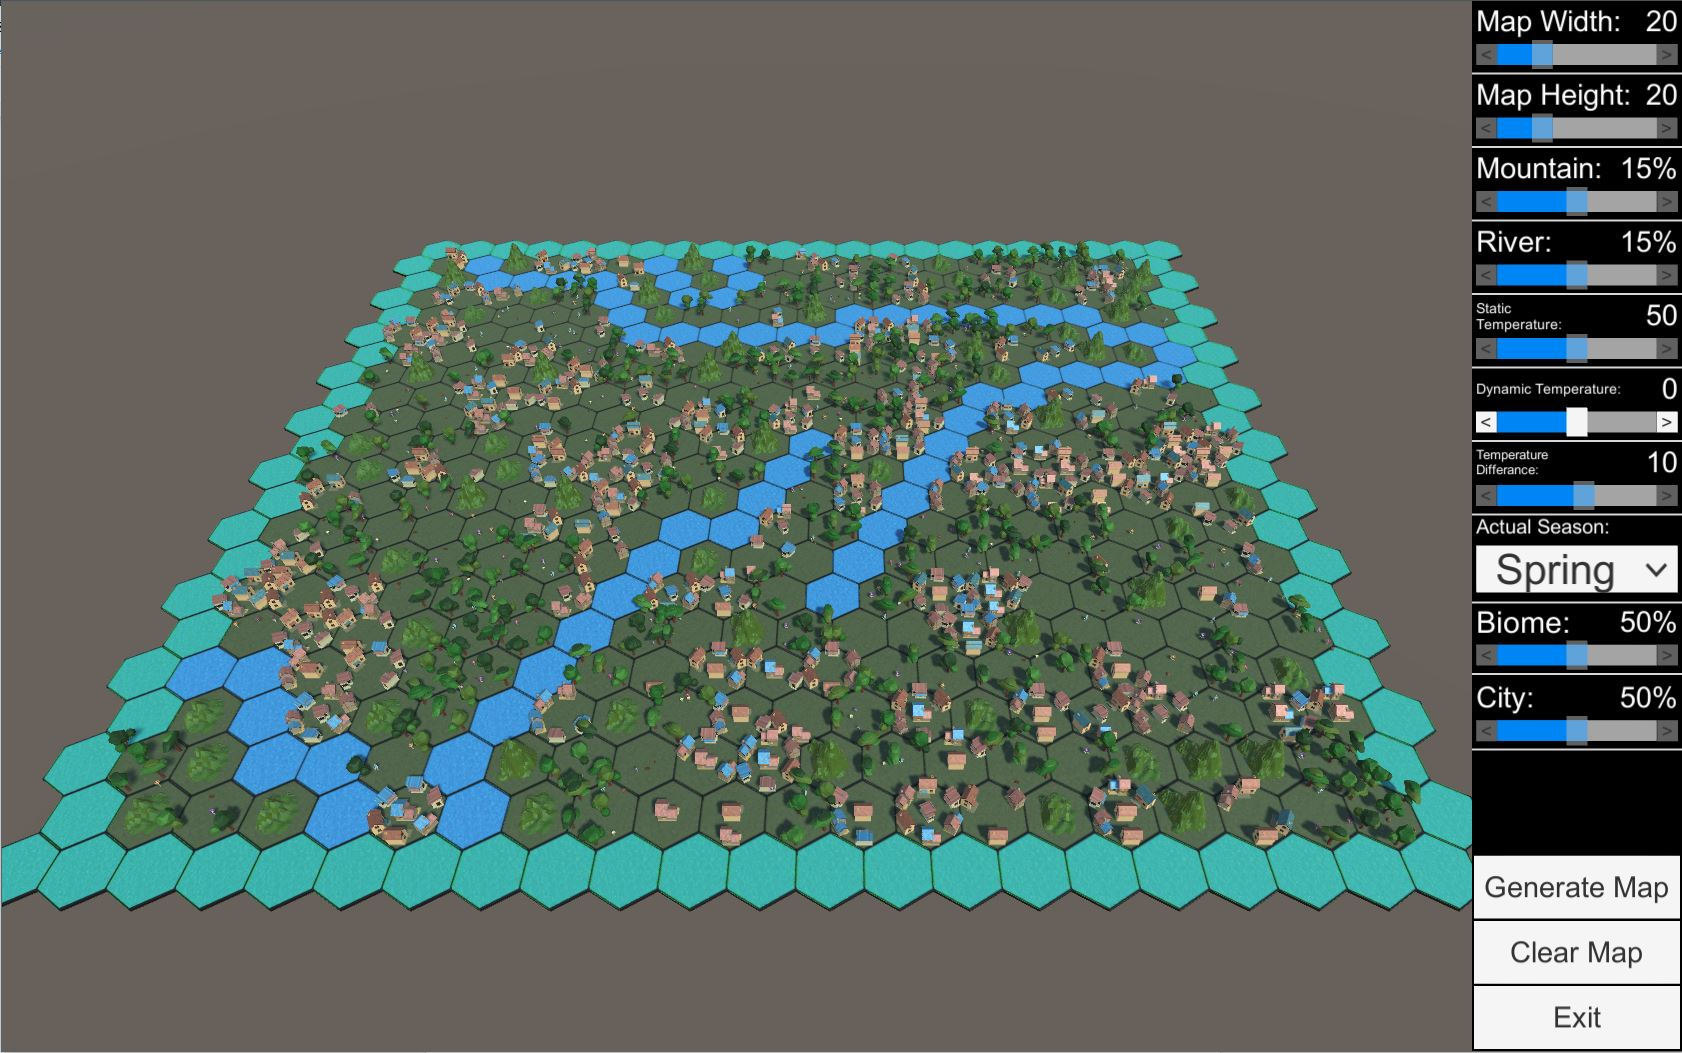
\includegraphics[scale=0.215]{kepek/UserGuide2.jpg}
\caption{A program grafikai beállítási lehetőségei}
\label{fig:UserGuide2}
\end{figure}

Beállítási lehetőségek (felülről lefelé):
\begin{itemize}
\item Térkép magassága,
\item Térkép szélessége,
\item Hegyek számossága a térkép méretének megfelelő arányban,
\item Folyók számossága a térkép méretének megfelelő arányban,
\item Statikus hőmérséklet,
\item Dinamikus hőmérséklet,
\item Hőmérséklet átmenet a térkép teteje és az alja között,
\item Évszakok beállítása,
\item A növényzet számossága a a térképen százalékban kifejezve,
\item A városok számossága a a térképen százalékban kifejezve.
\end{itemize}

A ,,Generate Map'' gomb megnyomására a kiválasztott beállításoknak a használatával az algoritmus létrehoz egy térképet. A ,,Clear Map'' gomb megnyomására a legenerált térkép tőrlődik. Az ,,Exit'' gomb megnyomására az alkalmazás bezárul.

\section*{Kamerakezelés}

\begin{itemize}
\item A \textit{W, A, S, D} billentyűk, a nyilak és az egér mozgatásával (miközben lenyomva tartjuk a görgőt) lehetséges mozgatni a kamerát a vízszintes tengelyek mentén.
\item A \textit{Q, E} gombok és az egér mozgatásával (jobb gomb lenyomvatartása közben) lehetséges forgatni a kamerát a vertikális tengely mentén.
\item Az \textit{R, F} gombok és az egér görgőjének a görgetésével lehet a kamera magasságát befolyásolni.
\end{itemize}
